\FChapter{Chapter Fifteen}{15}

\Lettrine{M}{r.\@} \textsc{ Rochester} did, on a future occasion, explain it. It was one
afternoon, when he chanced to meet me and Adèle in the grounds: and
while she played with Pilot and her shuttlecock, he asked me to walk up
and down a long beech avenue within sight of her.

He then said that she was the daughter of a French opera-dancer, Céline
Varens, towards whom he had once cherished what he called a
\foreignquote{french}{\emph{grande passion}.} This passion Céline had professed to return
with even superior ardour. He thought himself her idol, ugly as he was:
he believed, as he said, that she preferred his \foreignquote{french}{\emph{taille
d'athlète}}\footnote{\emph{\enquote{athletic build}}} to the elegance of the Apollo Belvidere.

\enquote{And, Miss Eyre, so much was I flattered by this preference of
the Gallic sylph for her British gnome, that I installed her in an
hotel; gave her a complete establishment of servants, a carriage,
cashmeres, diamonds, dentelles, \etc. In short, I began the process of
ruining myself in the received style, like any other spoony. I had not,
it seems, the originality to chalk out a new road to shame and
destruction, but trode the old track with stupid exactness not to
deviate an inch from the beaten centre. I had---as I deserved to
have---the fate of all other spoonies. Happening to call one evening
when Céline did not expect me, I found her out; but it was a warm night,
and I was tired with strolling through Paris, so I sat down in her
boudoir; happy to breathe the air consecrated so lately by her
presence. No,---I exaggerate; I never thought there was any
consecrating virtue about her: it was rather a sort of pastille perfume
she had left; a scent of musk and amber, than an odour of sanctity. I
was just beginning to stifle with the fumes of conservatory flowers and
sprinkled essences, when I bethought myself to open the window and step
out on to the balcony. It was moonlight and gaslight besides, and very
still and serene. The balcony was furnished with a chair or two; I sat
down, and took out a cigar,---I will take one now, if you will excuse
me.}

Here ensued a pause, filled up by the producing and lighting of a cigar;
having placed it to his lips and breathed a trail of Havannah incense on
the freezing and sunless air, he went on---

\enquote{I liked bonbons too in those days, Miss Eyre, and I was
\emph{croquant}---(overlook the barbarism)---\emph{croquant} chocolate %TODO french
comfits, and smoking alternately, watching meantime the equipages that
rolled along the fashionable streets towards the neighbouring
opera-house, when in an elegant close carriage drawn by a beautiful pair
of English horses, and distinctly seen in the brilliant city-night, I
recognised the \foreignquote{french}{voiture}\footnote{\enquote{carriage}} I had given Céline. She was
returning: of course my heart thumped with impatience against the iron
rails I leant upon. The carriage stopped, as I had expected, at the
hotel door; my flame (that is the very word for an opera inamorata)
alighted: though muffed in a cloak---an unnecessary encumbrance,
by-the-bye, on so warm a June evening---I knew her instantly by her
little foot, seen peeping from the skirt of her dress, as she skipped
from the carriage-step. Bending over the balcony, I was about to murmur
\foreignquote{french}{Mon ange}\footnote{\enquote{My angel}}---in a tone, of course, which should be audible to
the ear of love alone---when a figure jumped from the carriage after
her; cloaked also; but that was a spurred heel which had rung on the
pavement, and that was a hatted head which now passed under the arched
\foreignlanguage{french}{\emph{porte cochère}}\footnote{\emph{carriage porch}} of the hotel.

%removed enq
You never felt jealousy, did you, Miss Eyre? Of course not: I need
not ask you; because you never felt love. You have both sentiments yet
to experience: your soul sleeps; the shock is yet to be given which
shall waken it. You think all existence lapses in as quiet a flow as
that in which your youth has hitherto slid away. Floating on with
closed eyes and muffled ears, you neither see the rocks bristling not
far off in the bed of the flood, nor hear the breakers boil at their
base. But I tell you---and you may mark my words---you will come some
day to a craggy pass in the channel, where the whole of life's stream
will be broken up into whirl and tumult, foam and noise: either you will
be dashed to atoms on crag points, or lifted up and borne on by some
master-wave into a calmer current---as I am now.

%removed enq
I like this day; I like that sky of steel; I like the sternness
and stillness of the world under this frost. I like Thornfield, its
antiquity, its retirement, its old crow-trees and thorn-trees, its grey
façade, and lines of dark windows reflecting that metal welkin: and yet
how long have I abhorred the very thought of it, shunned it like a great
plague-house? How I do still abhor---}

He ground his teeth and was silent: he arrested his step and struck his
boot against the hard ground. Some hated thought seemed to have him in
its grip, and to hold him so tightly that he could not advance.

We were ascending the avenue when he thus paused; the hall was before
us. Lifting his eye to its battlements, he cast over them a glare such
as I never saw before or since. Pain, shame, ire, impatience, disgust,
detestation, seemed momentarily to hold a quivering conflict in the
large pupil dilating under his ebon eyebrow. Wild was the wrestle which
should be paramount; but another feeling rose and triumphed: something
hard and cynical: self-willed and resolute: it settled his passion and
petrified his countenance: he went on---

\enquote{During the moment I was silent, Miss Eyre, I was arranging a point
with my destiny. She stood there, by that beech-trunk---a hag like one
of those who appeared to Macbeth on the heath of Forres. \enquote{You
like Thornfield?} she said, lifting her finger; and then she wrote in
the air a memento, which ran in lurid hieroglyphics all along the
house-front, between the upper and lower row of windows, \enquote{Like
it if you can! Like it if you dare!}

%removed enq
\enquote{I will like it,} said I; \enquote{I dare like it;}
and} (he subjoined moodily) \enquote{I will keep my word; I will break
obstacles to happiness, to goodness---yes, goodness. I wish to be a
better man than I have been, than I am; as Job's leviathan broke the
spear, the dart, and the habergeon, hindrances which others count as
iron and brass, I will esteem but straw and rotten wood.}

Adèle here ran before him with her shuttlecock. \enquote{Away!} he
cried harshly; \enquote{keep at a distance, child; or go in to Sophie!} 
Continuing then to pursue his walk in silence, I ventured to recall him
to the point whence he had abruptly diverged---

\enquote{Did you leave the balcony, sir,} I asked, \enquote{when Mdlle.
Varens entered?}

I almost expected a rebuff for this hardly well-timed question, but, on
the contrary, waking out of his scowling abstraction, he turned his eyes
towards me, and the shade seemed to clear off his brow. \enquote{Oh, I
had forgotten Céline! Well, to resume. When I saw my charmer thus come
in accompanied by a cavalier, I seemed to hear a hiss, and the green
snake of jealousy, rising on undulating coils from the moonlit balcony,
glided within my waistcoat, and ate its way in two minutes to my heart's
core. Strange!} he exclaimed, suddenly starting again from the point. 
\enquote{Strange that I should choose you for the confidant of all this,
young lady; passing strange that you should listen to me quietly, as if
it were the most usual thing in the world for a man like me to tell
stories of his opera-mistresses to a quaint, inexperienced girl like
you! But the last singularity explains the first, as I intimated once
before: you, with your gravity, considerateness, and caution were made
to be the recipient of secrets. Besides, I know what sort of a mind I
have placed in communication with my own: I know it is one not liable to
take infection: it is a peculiar mind: it is a unique one. Happily I do
not mean to harm it: but, if I did, it would not take harm from me. The
more you and I converse, the better; for while I cannot blight you, you
may refresh me.} After this digression he proceeded---

\enquote{I remained in the balcony. \enquote{They will come to her boudoir,
no doubt,} thought I: \enquote{let me prepare an ambush.} So putting
my hand in through the open window, I drew the curtain over it, leaving
only an opening through which I could take observations; then I closed
the casement, all but a chink just wide enough to furnish an outlet to
lovers' whispered vows: then I stole back to my chair; and as I resumed
it the pair came in. My eye was quickly at the aperture. Céline's
chamber-maid entered, lit a lamp, left it on the table, and withdrew. 
The couple were thus revealed to me clearly: both removed their cloaks,
and there was \enquote{the Varens,} shining in satin and jewels,---my
gifts of course,---and there was her companion in an officer's uniform;
and I knew him for a young roué of a vicomte---a brainless and vicious
youth whom I had sometimes met in society, and had never thought of
hating because I despised him so absolutely. On recognising him, the
fang of the snake Jealousy was instantly broken; because at the same
moment my love for Céline sank under an extinguisher. A woman who could
betray me for such a rival was not worth contending for; she deserved
only scorn; less, however, than I, who had been her dupe.

%rem enq
They began to talk; their conversation eased me completely: frivolous,
mercenary, heartless, and senseless, it was rather calculated to weary
than enrage a listener. A card of mine lay on the table; this being
perceived, brought my name under discussion. Neither of them possessed
energy or wit to belabour me soundly, but they insulted me as coarsely
as they could in their little way: especially Céline, who even waxed
rather brilliant on my personal defects---deformities she termed them. 
Now it had been her custom to launch out into fervent admiration of what
she called my \foreignquote{french}{\emph{beauté mâle}:} wherein she differed diametrically
from you, who told me point-blank, at the second interview, that you did
not think me handsome. The contrast struck me at the time and---}

Adèle here came running up again.

\enquote{Monsieur, John has just been to say that your agent has called
and wishes to see you.}

\enquote{Ah! in that case I must abridge. Opening the window, I walked
in upon them; liberated Céline from my protection; gave her notice to
vacate her hotel; offered her a purse for immediate exigencies;
disregarded screams, hysterics, prayers, protestations, convulsions;
made an appointment with the vicomte for a meeting at the Bois de
Boulogne. Next morning I had the pleasure of encountering him; left a
bullet in one of his poor etiolated arms, feeble as the wing of a
chicken in the pip, and then thought I had done with the whole crew. 
But unluckily the Varens, six months before, had given me this filette
Adèle, who, she affirmed, was my daughter; and perhaps she may be,
though I see no proofs of such grim paternity written in her
countenance: Pilot is more like me than she. Some years after I had
broken with the mother, she abandoned her child, and ran away to Italy
with a musician or singer. I acknowledged no natural claim on Adèle's
part to be supported by me, nor do I now acknowledge any, for I am not
her father; but hearing that she was quite destitute, I e'en took the
poor thing out of the slime and mud of Paris, and transplanted it here,
to grow up clean in the wholesome soil of an English country garden. 
\Mrs{} Fairfax found you to train it; but now you know that it is the
illegitimate offspring of a French opera-girl, you will perhaps think
differently of your post and protégée: you will be coming to me some day
with notice that you have found another place---that you beg me to look
out for a new governess, \etc.---Eh?}

\enquote{No: Adèle is not answerable for either her mother's faults or
yours: I have a regard for her; and now that I know she is, in a sense,
parentless---forsaken by her mother and disowned by you, sir---I shall
cling closer to her than before. How could I possibly prefer the spoilt
pet of a wealthy family, who would hate her governess as a nuisance, to
a lonely little orphan, who leans towards her as a friend?}

\enquote{Oh, that is the light in which you view it! Well, I must go in
now; and you too: it darkens.}

But I stayed out a few minutes longer with Adèle and Pilot---ran a race
with her, and played a game of battledore and shuttlecock. When we went
in, and I had removed her bonnet and coat, I took her on my knee; kept
her there an hour, allowing her to prattle as she liked: not rebuking
even some little freedoms and trivialities into which she was apt to
stray when much noticed, and which betrayed in her a superficiality of
character, inherited probably from her mother, hardly congenial to an
English mind. Still she had her merits; and I was disposed to
appreciate all that was good in her to the utmost. I sought in her
countenance and features a likeness to \Mr{} Rochester, but found none: no
trait, no turn of expression announced relationship. It was a pity: if
she could but have been proved to resemble him, he would have thought
more of her.

It was not till after I had withdrawn to my own chamber for the night,
that I steadily reviewed the tale \Mr{} Rochester had told me. As he had
said, there was probably nothing at all extraordinary in the substance
of the narrative itself: a wealthy Englishman's passion for a French
dancer, and her treachery to him, were every-day matters enough, no
doubt, in society; but there was something decidedly strange in the
paroxysm of emotion which had suddenly seized him when he was in the act
of expressing the present contentment of his mood, and his newly revived
pleasure in the old hall and its environs. I meditated wonderingly on
this incident; but gradually quitting it, as I found it for the present
inexplicable, I turned to the consideration of my master's manner to
myself. The confidence he had thought fit to repose in me seemed a
tribute to my discretion: I regarded and accepted it as such. His
deportment had now for some weeks been more uniform towards me than at
the first. I never seemed in his way; he did not take fits of chilling
hauteur: when he met me unexpectedly, the encounter seemed welcome; he
had always a word and sometimes a smile for me: when summoned by formal
invitation to his presence, I was honoured by a cordiality of reception
that made me feel I really possessed the power to amuse him, and that
these evening conferences were sought as much for his pleasure as for my
benefit.

I, indeed, talked comparatively little, but I heard him talk with
relish. It was his nature to be communicative; he liked to open to a
mind unacquainted with the world glimpses of its scenes and ways (I do
not mean its corrupt scenes and wicked ways, but such as derived their
interest from the great scale on which they were acted, the strange
novelty by which they were characterised); and I had a keen delight in
receiving the new ideas he offered, in imagining the new pictures he
portrayed, and following him in thought through the new regions he
disclosed, never startled or troubled by one noxious allusion.

The ease of his manner freed me from painful restraint: the friendly
frankness, as correct as cordial, with which he treated me, drew me to
him. I felt at times as if he were my relation rather than my master:
yet he was imperious sometimes still; but I did not mind that; I saw it
was his way. So happy, so gratified did I become with this new interest
added to life, that I ceased to pine after kindred: my thin
crescent-destiny seemed to enlarge; the blanks of existence were filled
up; my bodily health improved; I gathered flesh and strength.

And was \Mr{}  Rochester now ugly in my eyes? No, reader: gratitude, and
many associations, all pleasurable and genial, made his face the object
I best liked to see; his presence in a room was more cheering than the
brightest fire. Yet I had not forgotten his faults; indeed, I could
not, for he brought them frequently before me. He was proud, sardonic,
harsh to inferiority of every description: in my secret soul I knew that
his great kindness to me was balanced by unjust severity to many
others. He was moody, too; unaccountably so; I more than once, when
sent for to read to him, found him sitting in his library alone, with
his head bent on his folded arms; and, when he looked up, a morose,
almost a malignant, scowl blackened his features. But I believed that
his moodiness, his harshness, and his former faults of morality (I say
\emph{former}, for now he seemed corrected of them) had their source in
some cruel cross of fate. I believed he was naturally a man of better
tendencies, higher principles, and purer tastes than such as
circumstances had developed, education instilled, or destiny
encouraged. I thought there were excellent materials in him; though for
the present they hung together somewhat spoiled and tangled. I cannot
deny that I grieved for his grief, whatever that was, and would have
given much to assuage it.

Though I had now extinguished my candle and was laid down in bed, I
could not sleep for thinking of his look when he paused in the avenue,
and told how his destiny had risen up before him, and dared him to be
happy at Thornfield.

\enquote{Why not?} I asked myself. \enquote{What alienates him from the
house? Will he leave it again soon? \Mrs{} Fairfax said he seldom stayed
here longer than a fortnight at a time; and he has now been resident
eight weeks. If he does go, the change will be doleful. Suppose he
should be absent spring, summer, and autumn: how joyless sunshine and
fine days will seem!}

I hardly know whether I had slept or not after this musing; at any rate,
I started wide awake on hearing a vague murmur, peculiar and lugubrious,
which sounded, I thought, just above me. I wished I had kept my candle
burning: the night was drearily dark; my spirits were depressed. I rose
and sat up in bed, listening. The sound was hushed.

I tried again to sleep; but my heart beat anxiously: my inward
tranquillity was broken. The clock, far down in the hall, struck two. 
Just then it seemed my chamber-door was touched; as if fingers had swept
the panels in groping a way along the dark gallery outside. I said,
\enquote{Who is there?} Nothing answered. I was chilled with fear.

All at once I remembered that it might be Pilot, who, when the
kitchen-door chanced to be left open, not unfrequently found his way up
to the threshold of \Mr{}  Rochester's chamber: I had seen him lying there
myself in the mornings. The idea calmed me somewhat: I lay down. 
Silence composes the nerves; and as an unbroken hush now reigned again
through the whole house, I began to feel the return of slumber. But it
was not fated that I should sleep that night. A dream had scarcely
approached my ear, when it fled affrighted, scared by a marrow-freezing
incident enough.

This was a demoniac laugh---low, suppressed, and deep---uttered, as it
seemed, at the very keyhole of my chamber door. The head of my bed was
near the door, and I thought at first the goblin-laugher stood at my
bedside---or rather, crouched by my pillow: but I rose, looked round,
and could see nothing; while, as I still gazed, the unnatural sound was
reiterated: and I knew it came from behind the panels. My first impulse
was to rise and fasten the bolt; my next, again to cry out, \enquote{Who
is there?}

Something gurgled and moaned. Ere long, steps retreated up the gallery
towards the third-storey staircase: a door had lately been made to shut
in that staircase; I heard it open and close, and all was still.

\enquote{Was that Grace Poole? and is she possessed with a devil?}
thought I\@. Impossible now to remain longer by myself: I must go to \Mrs{}
Fairfax. I hurried on my frock and a shawl; I withdrew the bolt and
opened the door with a trembling hand. There was a candle burning just
outside, and on the matting in the gallery. I was surprised at this
circumstance: but still more was I amazed to perceive the air quite dim,
as if filled with smoke; and, while looking to the right hand and left,
to find whence these blue wreaths issued, I became further aware of a
strong smell of burning.

Something creaked: it was a door ajar; and that door was \Mr{}
 Rochester's, and the smoke rushed in a cloud from thence. I thought no
more of \Mrs{} Fairfax; I thought no more of Grace Poole, or the laugh: in
an instant, I was within the chamber. Tongues of flame darted round the
bed: the curtains were on fire. In the midst of blaze and vapour, \Mr{}
 Rochester lay stretched motionless, in deep sleep.

\enquote{Wake! wake!} I cried. I shook him, but he only murmured and
turned: the smoke had stupefied him. Not a moment could be lost: the
very sheets were kindling, I rushed to his basin and ewer; fortunately,
one was wide and the other deep, and both were filled with water. I
heaved them up, deluged the bed and its occupant, flew back to my own
room, brought my own water-jug, baptized the couch afresh, and, by God's
aid, succeeded in extinguishing the flames which were devouring it.

The hiss of the quenched element, the breakage of a pitcher which I
flung from my hand when I had emptied it, and, above all, the splash of
the shower-bath I had liberally bestowed, roused \Mr{}  Rochester at last. 
Though it was now dark, I knew he was awake; because I heard him
fulminating strange anathemas at finding himself lying in a pool of
water.

\enquote{Is there a flood?} he cried.

\enquote{No, sir,} I answered; \enquote{but there has been a fire: get
up, do; you are quenched now; I will fetch you a candle.}

\enquote{In the name of all the elves in Christendom, is that Jane
Eyre?} he demanded. \enquote{What have you done with me, witch,
sorceress? Who is in the room besides you? Have you plotted to drown
me?}

\enquote{I will fetch you a candle, sir; and, in Heaven's name, get up. 
Somebody has plotted something: you cannot too soon find out who and
what it is.}

\enquote{There! I am up now; but at your peril you fetch a candle yet:
wait two minutes till I get into some dry garments, if any dry there
be---yes, here is my dressing-gown. Now run!}

I did run; I brought the candle which still remained in the gallery. He
took it from my hand, held it up, and surveyed the bed, all blackened
and scorched, the sheets drenched, the carpet round swimming in water.

\enquote{What is it? and who did it?} he asked. I briefly related to
him what had transpired: the strange laugh I had heard in the gallery:
the step ascending to the third storey; the smoke,---the smell of fire
which had conducted me to his room; in what state I had found matters
there, and how I had deluged him with all the water I could lay hands
on.

\begin{figure}
	\begin{sidecaption}{\enquote{What is it?\linebreak and who did it?}\linebreak he asked.}[p140b]
		\centering
		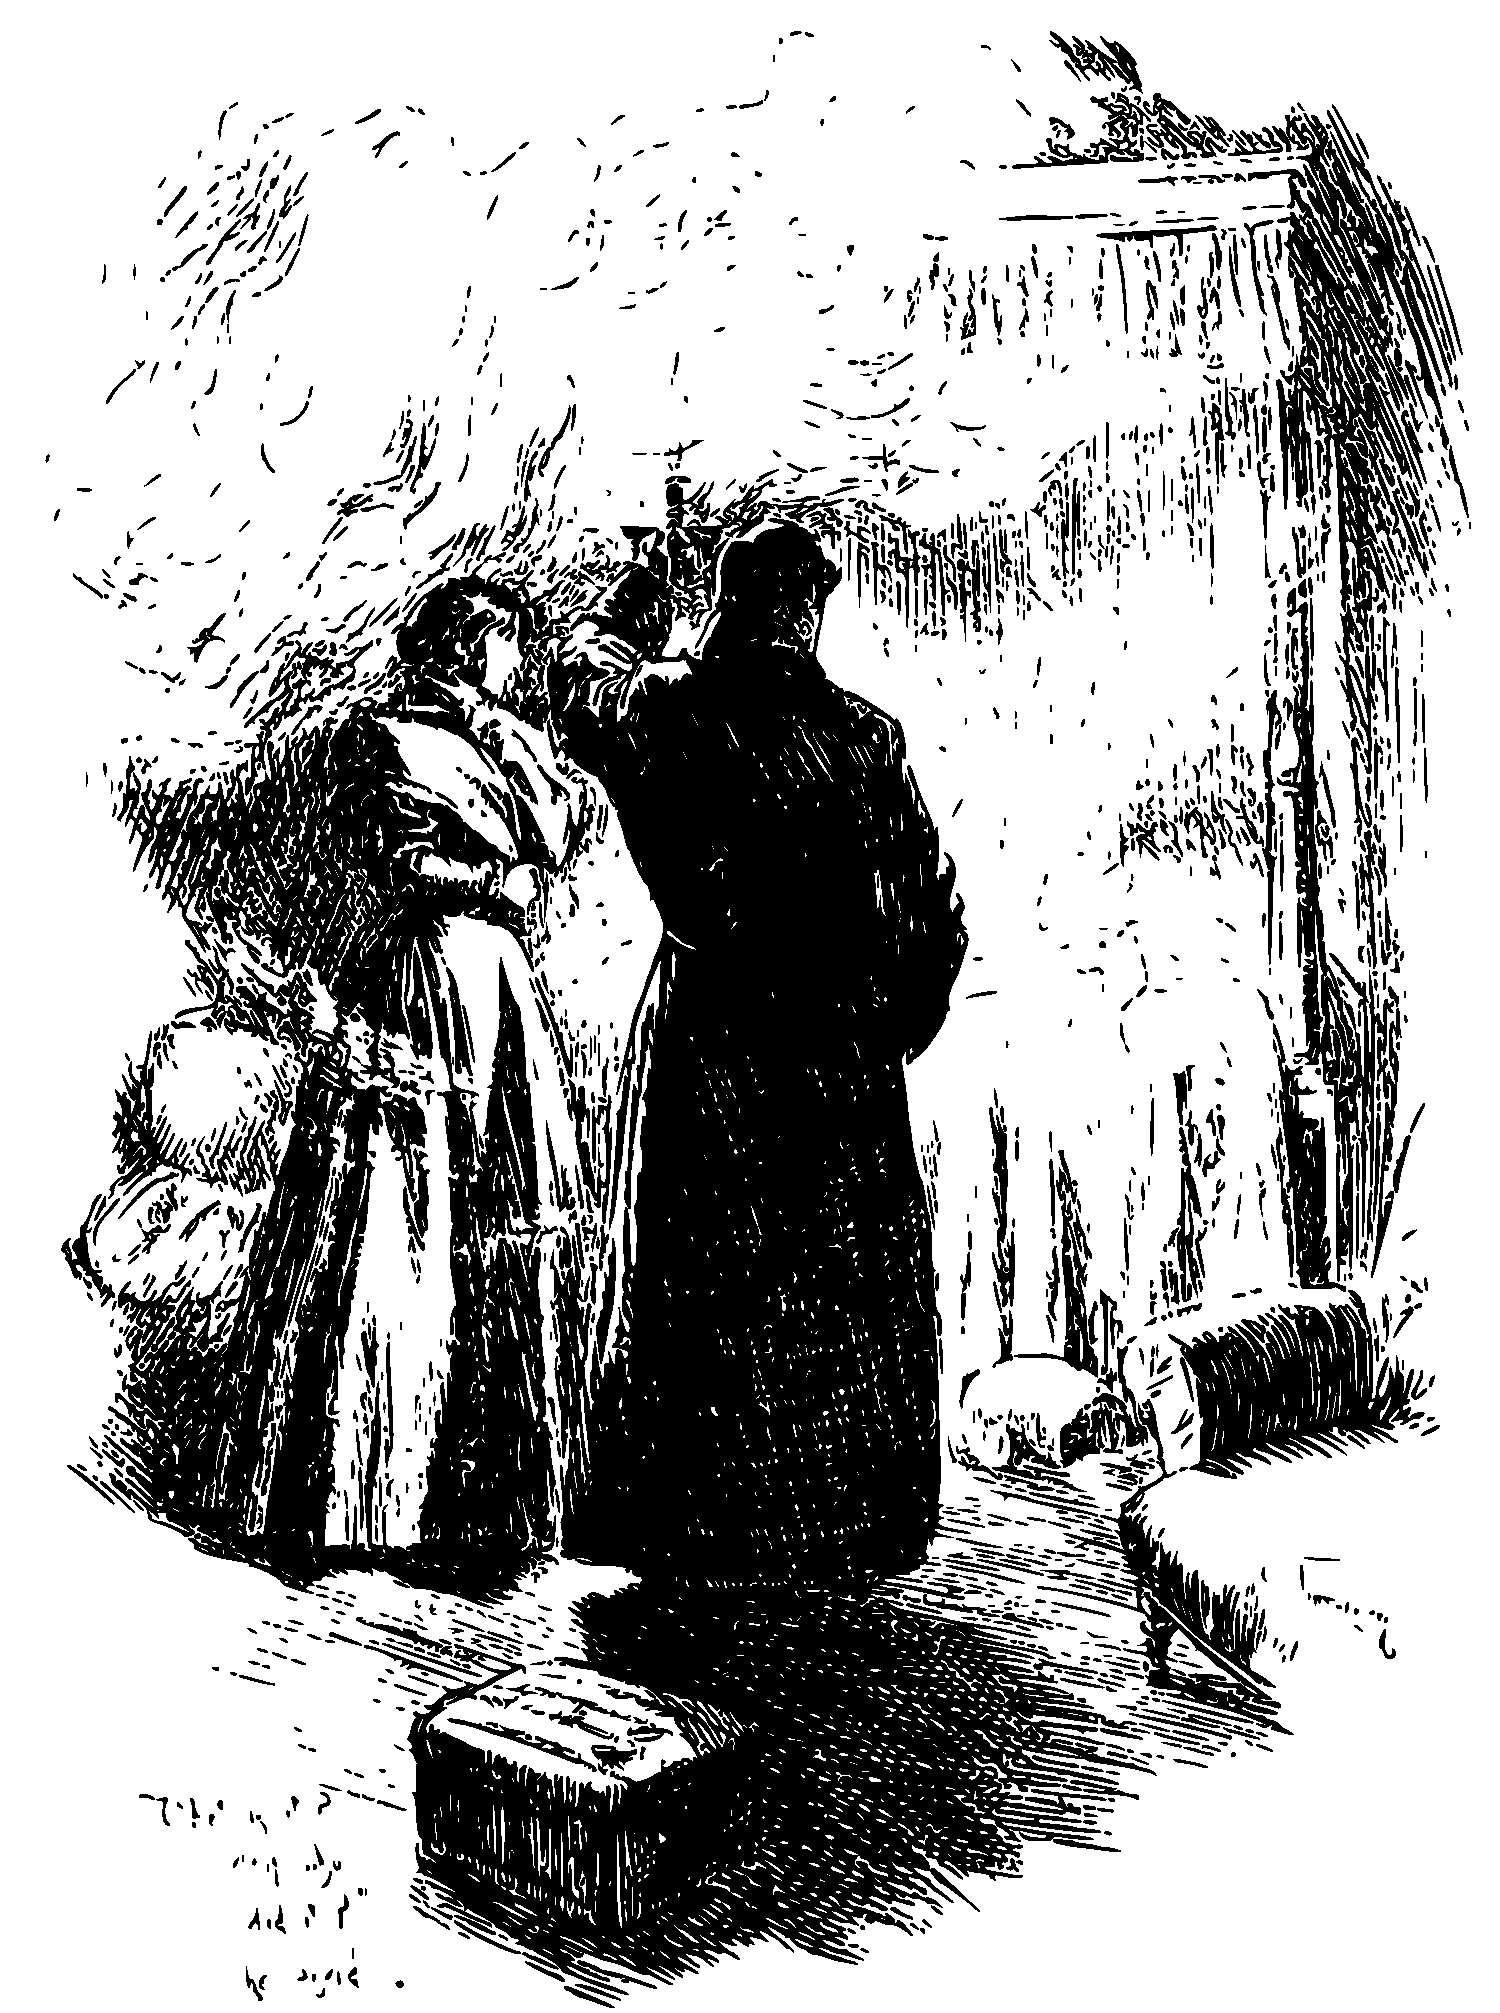
\includegraphics[width=\linewidth]{images/p140b.pdf}
	\end{sidecaption}
\end{figure}

He listened very gravely; his face, as I went on, expressed more concern
than astonishment; he did not immediately speak when I had concluded.

\enquote{Shall I call \Mrs{} Fairfax?} I asked.

\enquote{\Mrs{} Fairfax? No; what the deuce would you call her for? What
can she do? Let her sleep unmolested.}

\enquote{Then I will fetch Leah, and wake John and his wife.}

\enquote{Not at all: just be still. You have a shawl on. If you are
not warm enough, you may take my cloak yonder; wrap it about you, and
sit down in the arm-chair: there,---I will put it on. Now place your
feet on the stool, to keep them out of the wet. I am going to leave you
a few minutes. I shall take the candle. Remain where you are till I
return; be as still as a mouse. I must pay a visit to the second
storey. Don't move, remember, or call any one.}

He went: I watched the light withdraw. He passed up the gallery very
softly, unclosed the staircase door with as little noise as possible,
shut it after him, and the last ray vanished. I was left in total
darkness. I listened for some noise, but heard nothing. A very long
time elapsed. I grew weary: it was cold, in spite of the cloak; and
then I did not see the use of staying, as I was not to rouse the house. 
I was on the point of risking \Mr{}  Rochester's displeasure by disobeying
his orders, when the light once more gleamed dimly on the gallery wall,
and I heard his unshod feet tread the matting. \enquote{I hope it is
he,} thought I, \enquote{and not something worse.}

He re-entered, pale and very gloomy. \enquote{I have found it all out,}
said he, setting his candle down on the washstand; \enquote{it is as I
thought.}

\enquote{How, sir?}

He made no reply, but stood with his arms folded, looking on the
ground. At the end of a few minutes he inquired in rather a peculiar
tone---

\enquote{I forget whether you said you saw anything when you opened your
chamber door.}

\enquote{No, sir, only the candlestick on the ground.}

\enquote{But you heard an odd laugh? You have heard that laugh before,
I should think, or something like it?}

\enquote{Yes, sir: there is a woman who sews here, called Grace
Poole,---she laughs in that way. She is a singular person.}

\enquote{Just so. Grace Poole---you have guessed it. She is, as you
say, singular---very. Well, I shall reflect on the subject. Meantime,
I am glad that you are the only person, besides myself, acquainted with
the precise details of to-night's incident. You are no talking fool:
say nothing about it. I will account for this state of affairs}
(pointing to the bed): \enquote{and now return to your own room. I
shall do very well on the sofa in the library for the rest of the
night. It is near four:---in two hours the servants will be up.}

\enquote{Good-night, then, sir,} said I, departing.

He seemed surprised---very inconsistently so, as he had just told me to
go.

\enquote{What!} he exclaimed, \enquote{are you quitting me already, and
in that way?}

\enquote{You said I might go, sir.}

\enquote{But not without taking leave; not without a word or two of
acknowledgment and good-will: not, in short, in that brief, dry
fashion. Why, you have saved my life!---snatched me from a horrible and
excruciating death! and you walk past me as if we were mutual
strangers! At least shake hands.}

He held out his hand; I gave him mine: he took it first in one, them in
both his own.

\enquote{You have saved my life: I have a pleasure in owing you so
immense a debt. I cannot say more. Nothing else that has being would
have been tolerable to me in the character of creditor for such an
obligation: but you: it is different;---I feel your benefits no burden,
Jane.}

He paused; gazed at me: words almost visible trembled on his lips,---but
his voice was checked.

\enquote{Good-night again, sir. There is no debt, benefit, burden,
obligation, in the case.}

\enquote{I knew,} he continued, \enquote{you would do me good in some
way, at some time;---I saw it in your eyes when I first beheld you:
their expression and smile did not}---(again he stopped)---\enquote{did
not} (he proceeded hastily) \enquote{strike delight to my very inmost
heart so for nothing. People talk of natural sympathies; I have heard
of good genii: there are grains of truth in the wildest fable. My
cherished preserver, goodnight!}

Strange energy was in his voice, strange fire in his look.

\enquote{I am glad I happened to be awake,} I said: and then I was
going.

\enquote{What! you \emph{will} go?}

\enquote{I am cold, sir.}

\enquote{Cold? Yes,---and standing in a pool! Go, then, Jane; go!} 
But he still retained my hand, and I could not free it. I bethought
myself of an expedient.

\enquote{I think I hear \Mrs{} Fairfax move, sir,} said I\@.

\enquote{Well, leave me:} he relaxed his fingers, and I was gone.

I regained my couch, but never thought of sleep. Till morning dawned I
was tossed on a buoyant but unquiet sea, where billows of trouble rolled
under surges of joy. I thought sometimes I saw beyond its wild waters a
shore, sweet as the hills of Beulah; and now and then a freshening gale,
wakened by hope, bore my spirit triumphantly towards the bourne: but I
could not reach it, even in fancy---a counteracting breeze blew off
land, and continually drove me back. Sense would resist delirium:
judgment would warn passion. Too feverish to rest, I rose as soon as
day dawned.
